\newpage
\onecolumn
\appendix

\section{Case Study}
\label{appendix:cases}

We conduct a case study that demonstrates our approach can mitigate logical errors in code generation. Figure~\ref{fig:case_study} presents the number-of-black-blocks problem, where different methods exhibit distinct enumeration strategies. The base model incorrectly iterates with ranges that miss left and top blocks while over-counting right and bottom ones. GRPO partially improves but still uses incorrect ranges for $i \in \text{range}(\max(0, x - 1), \min(m - 1, x + 1) + 1)$, leading to overcounting. In contrast, our proposed \ourapproach correctly identifies that for each black cell at position $(x, y)$, it can belong to at most 4 possible $2 \times 2$ blocks, and properly implements the enumeration logic by checking the valid range boundaries, ensuring accurate counting without missing or double-counting any blocks. This demonstrates \ourapproach's effectiveness in learning precise logical patterns for code generation tasks.

\begin{figure*}[h!] 
    \centering 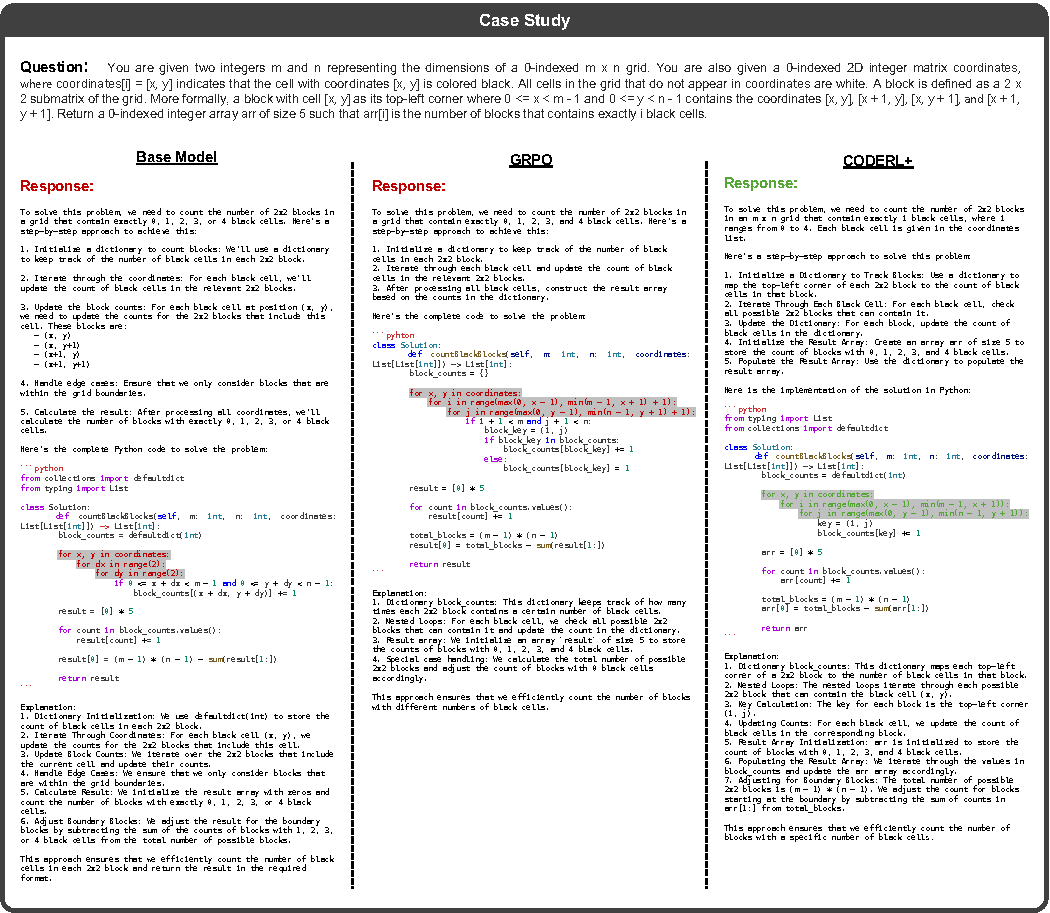
\includegraphics[width=\textwidth]{figures/cases.pdf} 
    \caption{Cases of base model (Qwen2.5-Coder-7B-Instruct), GRPO, and \ourapproach.} 
    \label{fig:case_study} 
\end{figure*}

\section{Setup of Probe Analyses}\label{probe_setup}

This experiment is based on the HumanEval code generation dataset and investigates three models: Base Model (Qwen2.5-Coder-7B-Instruct), GRPO, and \ourapproach. We first process the original dataset by decomposing each task, which contains multiple test cases, into several "single-example" tasks where each prompt includes only one input-output example. Subsequently, for each original task, we randomly split all its corresponding sub-tasks into a training set and a test set for the probe, using an 8:2 ratio.

Our experimental pipeline follows a "generate-execute-extract" paradigm. First, we prompt the three models to generate Python code for each single-example prompt. Next, we execute the generated code with its corresponding input example, capturing and recording the final values of all numerical intermediate variables within the function upon its completion. Finally, we feed the generated code back into its respective model, identify the token corresponding to the last occurrence of each traced variable, and extract the hidden state vector for that token from all model layers to serve as input features for the probe.

We train an independent linear regression model as a probe for each layer of each model. Given that the intermediate variables can vary significantly, we preprocess the data by normalizing the target variable values on a per-problem basis using Min-Max scaling to the range [-1, 1]. The normalization parameters are computed exclusively from the training set. All probes are trained for 10 epochs using the Adam optimizer with a learning rate of 1e-3, minimizing the Mean Squared Error (MSE) loss. For evaluation, our metric is the MSE in the normalized space on the test set. A lower MSE value indicates a better alignment between the model's internal representations and the code's execution semantics.

\section{Experiment Setup of Execution Trace Inference Task.}

We evaluate on the LiveCodeBench Code Reasoning task with an extended dataset. While the original task requires predicting a function's return value given its input and code, we extend it to also predict the final value of each intermediate variable at the end of its lifetime. This extension enables us to assess the model's understanding of code execution traces.
Specifically, we leverage the existing inputs and code from the LiveCodeBench Code Reasoning task, execute the code, and extract intermediate variables along with their final values at the end of their respective lifetimes.
The evaluated models include: Base Model (Qwen2.5-Coder-7B-Instruct), GRPO, and \ourapproach.
We use Exact@1 as the evaluation metric, which measures the proportion of cases where all intermediate variables and the final function return value are correctly predicted.
The evaluation prompt is as follows, where variables in blue are to be replaced with actual content:

\begin{promptbox}{Execution Trace Inference Task}
Given the following Python Code and Input, predict:

1) The code's output value (final\_output).

2) The final values of the listed local variables at the moment the code outputs.
\\\\
Python code: \verb|```python|\textcolor{blue}{\{code\}}\verb|```|

Input: \textcolor{blue}{\{test\_input\}}

Target local variables: \textcolor{blue}{\{local\_variable\_name\}}
\\\\
\textit{Instructions:}

1. First, write a reasoning section explaining step-by-step how the code executes with the given Input.

2. Do not include any JSON in the reasoning section.

3. On the LAST line only, output a strict JSON object with the required format. Example of final answer (LAST line only):
\{"final\_output": 3, "variables": \{"cnt": 2, "buf": [1, 2]\}\}
\end{promptbox}

\section{Implementation Details of Execution Semantics Alignment}
In implementation, the variable set $V$ is restricted to variables of primitive types (\eg, integers, floats, and strings), whose values can be deterministically represented and compared for reward computation. The ground-truth variable states $\mathcal{F}_{p_{\text{fail}}}(x)$ are obtained by executing the program and capturing the final values of target variables upon termination\footnote{The variable state extraction can be integrated into the existing execution process used for computing code generation rewards, requiring only a single execution per program and thus introducing minimal overhead.}. Furthermore, programs that encounter runtime errors are filtered out, as they do not yield valid execution trajectories. Only programs with semantic errors, \ie, code that executes normally but produces incorrect outputs, are selected for alignment. Such semantic errors represent the majority of code generation errors in LLMs.

\section{Additional Benchmark Results}\label{appendix:additional_benchmarks}

To further evaluate the generalizability of \ourapproach, we conduct additional experiments on two more code generation benchmarks: MBPP~\citep{mbpp} and LiveBench~\citep{livebench}. As shown in Table~\ref{tab:additional_benchmarks}, our method consistently outperforms the base model and GRPO baseline on both datasets in terms of pass@1, demonstrating that \ourapproach generalizes well beyond the primary evaluation benchmarks.

\begin{table}[h]
\centering
\caption{Performance of \ourapproach on additional code generation benchmarks.}
\begin{tabular}{lcc}
\toprule
Approach & MBPP & LiveBench \\
\midrule
Qwen2.5-Coder-7B-Instruct & 70.7 & 46.4 \\
GRPO & 72.1 & 46.9 \\
\ourapproach & \textbf{76.2} & \textbf{50.6} \\
\bottomrule
\end{tabular}\label{tab:additional_benchmarks}
\end{table}


\section{Limitations}
Our work has three limitations. First, computational constraints limited our evaluation to models up to 8B parameters, which may affect the generalizability of our conclusions to larger-scale LLMs. Second, we did not perform hyperparameter tuning due to the high computational cost of RL post-training, as each training run requires roughly three days. We followed prior work for training-related hyperparameters and empirically set the single hyperparameter specific to our method, maintaining this configuration across all experiments where it consistently yielded improvements. Third, while the execution semantics alignment component incurs additional computational overhead compared to standard RL algorithms, our experiments demonstrate that our approach achieves superior performance within comparable computational budgets (measured by training steps) and reaches higher performance ceilings as training progresses.
